\documentclass[final]{beamer}
\usepackage[orientation=landscape, size=a0, scale=1.0]{beamerposter}
\usepackage[utf8]{inputenc}
\usepackage[T1]{fontenc}
\usepackage{lmodern}
\usepackage{amsmath,amssymb}
\usepackage{booktabs}
\usepackage{graphicx}
\usepackage{enumitem}
\usepackage{xcolor}
\usepackage{colortbl}

\definecolor{shanghaitech}{RGB}{100, 30, 60}
\definecolor{lightbg}{RGB}{245, 240, 245}
\definecolor{darktext}{RGB}{30, 30, 30}
\definecolor{accentblue}{RGB}{40, 80, 140}
\definecolor{softgray}{RGB}{235, 235, 240}

\setbeamercolor{block title}{fg=white, bg=shanghaitech}
\setbeamercolor{block body}{fg=darktext, bg=lightbg}
\setbeamercolor{block alerted title}{fg=white, bg=accentblue}
\setbeamercolor{block alerted body}{fg=darktext, bg=lightbg}
\setbeamercolor{headline}{bg=shanghaitech}
\setbeamercolor{footline}{bg=shanghaitech, fg=white}
\setbeamertemplate{navigation symbols}{}

% Compact blocks
\setbeamertemplate{block begin}{%
  \vskip0.15em%
  \begin{beamercolorbox}[rounded=true,shadow=false,leftskip=0.4em,colsep*=0.3em]{block title}%
    \usebeamerfont{block title}\insertblocktitle%
  \end{beamercolorbox}%
  \vskip0.08em%
  \usebeamerfont{block body}%
  \begin{beamercolorbox}[rounded=true,shadow=false,colsep*=0.3em,sep=0.25em,vmode]{block body}%
}
\setbeamertemplate{block end}{%
  \end{beamercolorbox}\vskip0.15em%
}
\setbeamertemplate{block alerted begin}{%
  \vskip0.15em%
  \begin{beamercolorbox}[rounded=true,shadow=false,leftskip=0.4em,colsep*=0.3em]{block alerted title}%
    \usebeamerfont{block alerted title}\insertblocktitle%
  \end{beamercolorbox}%
  \vskip0.08em%
  \usebeamerfont{block alerted body}%
  \begin{beamercolorbox}[rounded=true,shadow=false,colsep*=0.3em,sep=0.25em,vmode]{block alerted body}%
}
\setbeamertemplate{block alerted end}{%
  \end{beamercolorbox}\vskip0.15em%
}

\graphicspath{{../../line_network_model/output/}{./}}

\begin{document}
\begin{frame}[t]
\vspace{-0.5cm}

% ================================================================
%  TITLE
% ================================================================
\begin{beamercolorbox}[wd=\paperwidth, center, sep=0.6cm]{headline}
{\fontsize{52}{58}\selectfont\bfseries\color{white} Reproducing Classical Heuristics for Urban Rail Transit Line Planning}\\[0.2cm]
{\fontsize{24}{28}\selectfont\color{white} Laporte et al.\ 2005 \quad$\cdot$\quad Ahmed et al.\ 2020}\\[0.12cm]
{\fontsize{16}{20}\selectfont\color{white} Zaizhou Yang \quad Yuzhou Lu \quad Jingrong Guan \quad$\vert$\quad
ShanghaiTech University \quad$\vert$\quad CS240: Algorithm Design and Analysis \quad$\vert$\quad Spring 2026}
\end{beamercolorbox}

\vspace{0.2cm}

% ================================================================
%  LEFT COLUMN (48%)
% ================================================================
\noindent
\begin{minipage}[t]{0.48\paperwidth}\normalsize

\begin{block}{\Large Motivation \& Problem}
\normalsize
The \textbf{Transit Network Design Problem} (TNDP) decides where to build stations and how to connect them in urban rail networks.
\begin{itemize}[leftmargin=*, label=\textcolor{shanghaitech}{$\blacktriangleright$}, itemsep=0.08em, parsep=0pt]
    \item \textbf{Objective:} maximize trip coverage \emph{or} minimize total system cost (passenger + operator + community)
    \item \textbf{Constraints:} construction budget, station spacing, geometric feasibility, connectivity
    \item \textbf{Complexity:} NP-hard (generalizes bounded-length Hamiltonian path)
\end{itemize}
We reproduce two representative algorithms on a \textbf{54-station candidate set} in central Shanghai, selected from OpenStreetMap population, job, transport, and commercial data layers.
\end{block}

\vspace{0.15cm}

\begin{block}{\Large Paper 1: Laporte 2005 --- Single-Line Trip Coverage}
\normalsize
\textbf{MTCP (Maximal Trip Coverage Problem):} Build one non-intersecting transit path through candidate stations to maximize OD demand coverage under a length budget $L_{\max}$:

$\displaystyle\max \sum_{(i,j) \in \mathcal{W}} f_{ij} \cdot y_{ij}$ \quad subject to $\sum_{e \in P} \ell_e \leq L_{\max}$, $P$ is a simple path.

\textbf{H1: Greedy Extension} \hfill {\small$O(n^2 \cdot |E|^2)$}

Start from a seed edge $(u,v)$. At each step, evaluate the marginal coverage gain of appending each unselected node at either endpoint. Greedily pick the best extension. Repeat until the length budget is exhausted.

\textbf{H2: Greedy Insertion} \hfill {\small$O(n^2 \cdot |E|^3)$}

Start from a seed edge. At each step, evaluate the marginal gain of inserting each unselected node at \emph{every} position in the current path. Three selection variants: \textbf{H2-A} (max ridership), \textbf{H2-B} (min length), \textbf{H2-C} (max ridership/length ratio).

\textbf{Post-optimization:} Iterative local search --- for each edge in the current path, test all possible swap replacements to improve coverage without increasing length.
\end{block}

\vspace{0.15cm}

\begin{block}{\Large Paper 2: Ahmed 2020 --- Multi-Line Network Design}
\normalsize
Unlike Laporte's single-line model, Ahmed 2020 addresses the \textbf{simultaneous design of multiple transit lines}:

$\displaystyle\min \;\; \phi_p \cdot C_{\mathrm{passenger}} + \phi_o \cdot C_{\mathrm{operator}} + \phi_c \cdot C_{\mathrm{community}}$

where $C_{\mathrm{passenger}}$ = travel time savings vs.\ car/bus, $C_{\mathrm{operator}}$ = operating cost savings from mode shift, $C_{\mathrm{community}}$ = construction cost (alignment length $\times$ per-km cost + stations $\times$ per-station cost).

\textbf{Two-stage approach:} (1) GIS-based feasibility screening to identify the candidate station pool; (2) Genetic Algorithm to simultaneously optimize station selection and line routing.

\textbf{GA operators:} Tournament selection (size 2), uniform crossover ($P_c = 0.7$) with feasibility repair, station-level mutation ($P_m = 0.3$).

\textbf{Chromosome encoding:} \texttt{[Line\_1: [terminal\_A, station\_seq, terminal\_B], Line\_2: ...]} --- each gene is a station index from the candidate pool.

\textbf{Constraints:} 4--10 stations/line, 1000--3000m station spacing, max 30\% line overlap, $\geq$1 transfer station per line.
\end{block}

\vspace{0.15cm}

\begin{block}{\Large Complexity Summary}
\normalsize
\begin{center}
\small
\begin{tabular}{@{}lcc@{}}
\toprule
\textbf{Algorithm} & \textbf{Per-Iteration} & \textbf{Total Worst-Case} \\
\midrule
H1 (Laporte) & $O(n \cdot |E|^2)$ & $O(n^2 \cdot |E|^2)$ \\
H2-A/B/C (Laporte) & $O(n \cdot |E|^3)$ & $O(n^2 \cdot |E|^3)$ \\
Post-optimization & $O(|E|^2 \cdot n)$/pass & $O(|E|^3 \cdot n)$ \\
Ahmed GA (per gen) & $O(L \cdot N_s^2 \log N_s)$ & $O(G \cdot P \cdot L \cdot N_s^2 \log N_s)$ \\
\bottomrule
\end{tabular}
\end{center}
Despite the underlying NP-hardness, all four algorithmic approaches run in \textbf{polynomial time}.
\end{block}

\vspace{0.15cm}

\begin{block}{\Large Key Conclusions}
\begin{enumerate}[leftmargin=*, label=\textcolor{shanghaitech}{\textbf{\arabic*.}}, itemsep=0.1em, parsep=0pt]
    \item \textbf{H2 insertion outperforms H1 extension} in OD coverage (54--57\% vs.\ 28\%), but H1 is 25$\times$ faster at scale. Trade-off: H1 for rapid screening, H2 for detailed design.
    \item \textbf{Simultaneous multi-line optimization} beats individual line design by \textbf{18\%}, confirming that global coordination of transfers and routing yields better networks.
    \item \textbf{Greedy-OD baseline} is surprisingly competitive with GA (56.5\% OD coverage at $<$0.01s), suggesting simple heuristics are near-optimal for single-objective scenarios.
    \item \textbf{Polynomial runtime scaling} confirmed empirically: H1 $\sim$0.8s, H2 $\sim$20s at $n{=}100$, with clear trends matching complexity analysis.
    \item \textbf{Practical recommendation:} Use greedy heuristics (H1/H2/Greedy-OD) for rapid feasibility screening; deploy GA-based methods when multi-line coordination and cost trade-offs are needed.
\end{enumerate}
\end{block}

\end{minipage}
\hfill
% ================================================================
%  RIGHT COLUMN (50%)
% ================================================================
\begin{minipage}[t]{0.50\paperwidth}\normalsize

\begin{block}{\Large Comprehensive Method Comparison}
\normalsize
We evaluate \textbf{9 algorithms} spanning greedy heuristics, metaheuristics, and ILP baselines:
\begin{center}
\small
\begin{tabular}{@{}lcccccc@{}}
\toprule
\textbf{Method} & \textbf{Stn} & \textbf{Len (km)} & \textbf{OD Cov} & \textbf{Lines} & \textbf{Xfer} & \textbf{Time} \\
\midrule
\rowcolor{softgray} Laporte H1   & 18 & 59.8 & 27.9\% & 1 & 0 & 0.05s \\
\rowcolor{white}  Laporte H2-A & 31 & 59.9 & 54.0\% & 1 & 0 & 0.77s \\
\rowcolor{softgray} Laporte H2-C & 33 & 59.6 & \textbf{56.8\%} & 1 & 0 & 0.88s \\
\midrule
\rowcolor{white}  Ahmed 1-line & 14 & 37.0 & 29.8\% & 1 & 0 & 33.5s \\
\rowcolor{softgray} Ahmed 2-line & 23 & 85.7 & 48.9\% & 2 & 5 & 56.3s \\
\rowcolor{white}  Ahmed 3-line & 20 & 130.8 & 31.8\% & 3 & 5 & 58.1s \\
\midrule
\rowcolor{softgray} Greedy-OD    & 23 & 57.1 & 56.5\% & 3 & 10 & 0.01s \\
\rowcolor{white}  Greedy-BCR   & 10 & 15.7 & 27.3\% & 3 & 2 & 0.01s \\
\rowcolor{softgray} GA (line-pool) & 32 & 56.0 & 40.4\% & 3 & 2 & 0.90s \\
\bottomrule
\end{tabular}
\end{center}
\end{block}

\vspace{0.2cm}

% --- GA CONVERGENCE (3 big plots) ---
\begin{alertblock}{\Large GA Convergence Curves}
\begin{center}
\begin{minipage}{0.31\linewidth}\centering
\Large\textbf{1-line}\\[0.1cm]
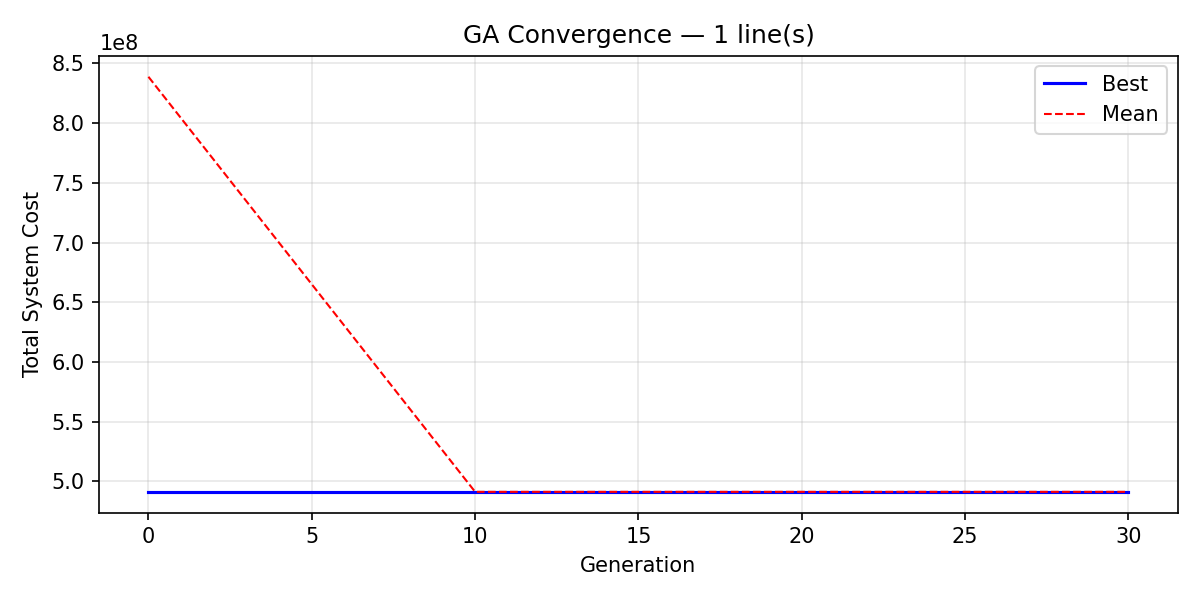
\includegraphics[width=\linewidth, height=10cm]{ahmed2020_reproduction/convergence_1line}\\[0.1cm]
{\normalsize 14 stations, 37.0 km}
\end{minipage}\hfill
\begin{minipage}{0.31\linewidth}\centering
\Large\textbf{2-line}\\[0.1cm]
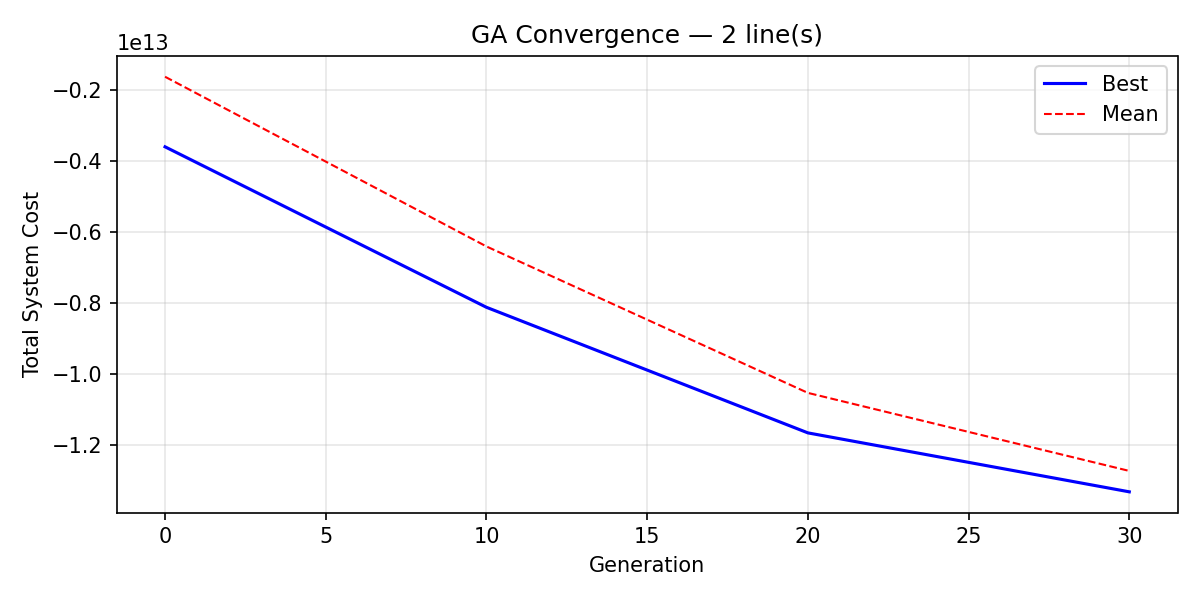
\includegraphics[width=\linewidth, height=10cm]{ahmed2020_reproduction/convergence_2line}\\[0.1cm]
{\normalsize 23 stations, 85.7 km}
\end{minipage}\hfill
\begin{minipage}{0.31\linewidth}\centering
\Large\textbf{3-line}\\[0.1cm]
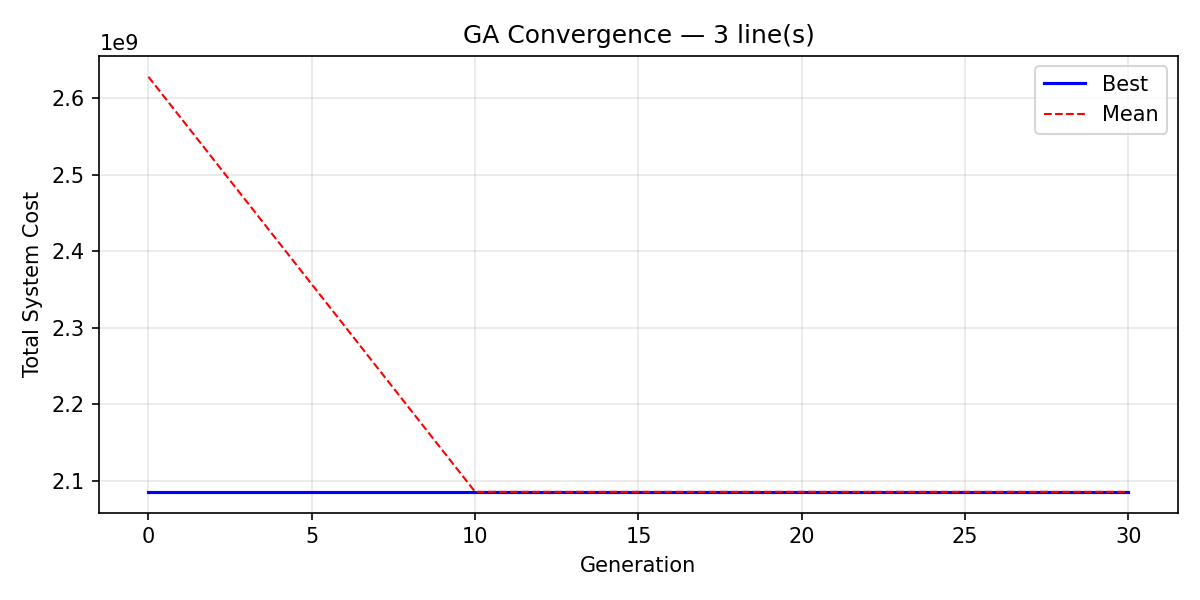
\includegraphics[width=\linewidth, height=10cm]{ahmed2020_reproduction/convergence_3line}\\[0.1cm]
{\normalsize 20 stations, 130.8 km}
\end{minipage}
\end{center}
\vspace{0.1cm}
{\normalsize All scenarios converge within 20--30 generations. The 2-line configuration achieves the lowest total cost ($-1.33\times10^{13}$), indicating that a well-coordinated two-line network captures more OD demand than either a single line or three competing lines.}
\end{alertblock}

\vspace{0.2cm}

% --- NETWORK VISUALIZATIONS (3 big maps) ---
\begin{block}{\Large Multi-Line Network Visualizations}
\begin{center}
\begin{minipage}{0.31\linewidth}\centering
\Large\textbf{1-line network}\\[0.1cm]
14 stations, 37.0 km\\[0.15cm]
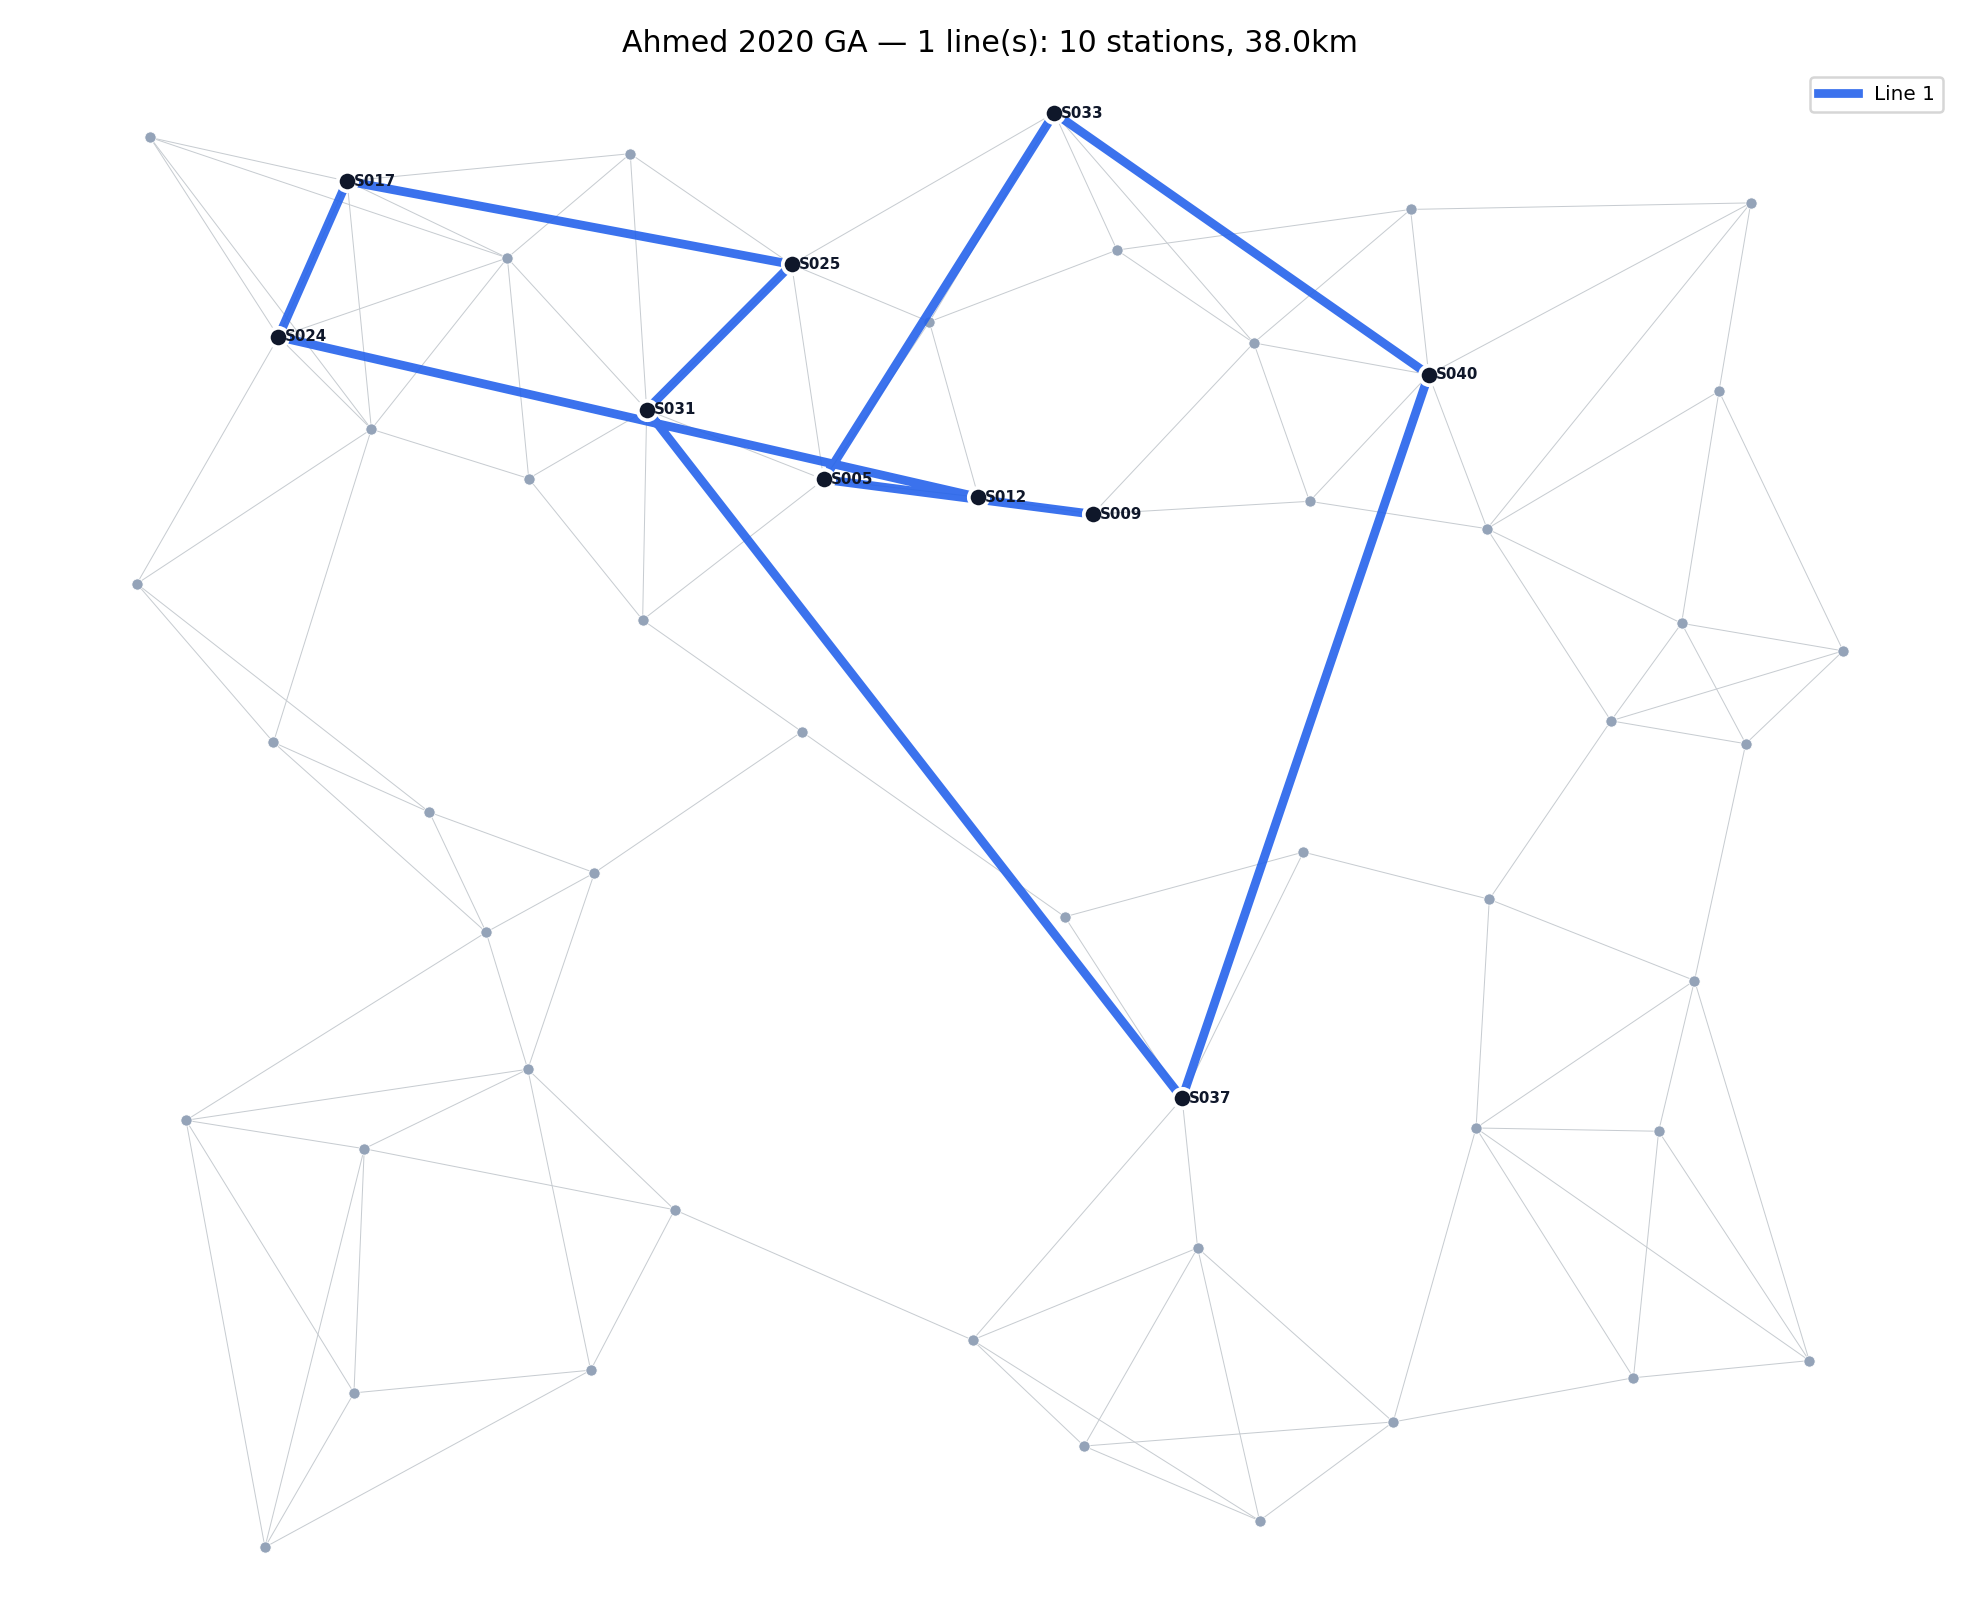
\includegraphics[width=\linewidth, height=14cm]{ahmed2020_reproduction/network_1line}
\end{minipage}\hfill
\begin{minipage}{0.31\linewidth}\centering
\Large\textbf{2-line network}\\[0.1cm]
23 stations, 85.7 km\\[0.15cm]
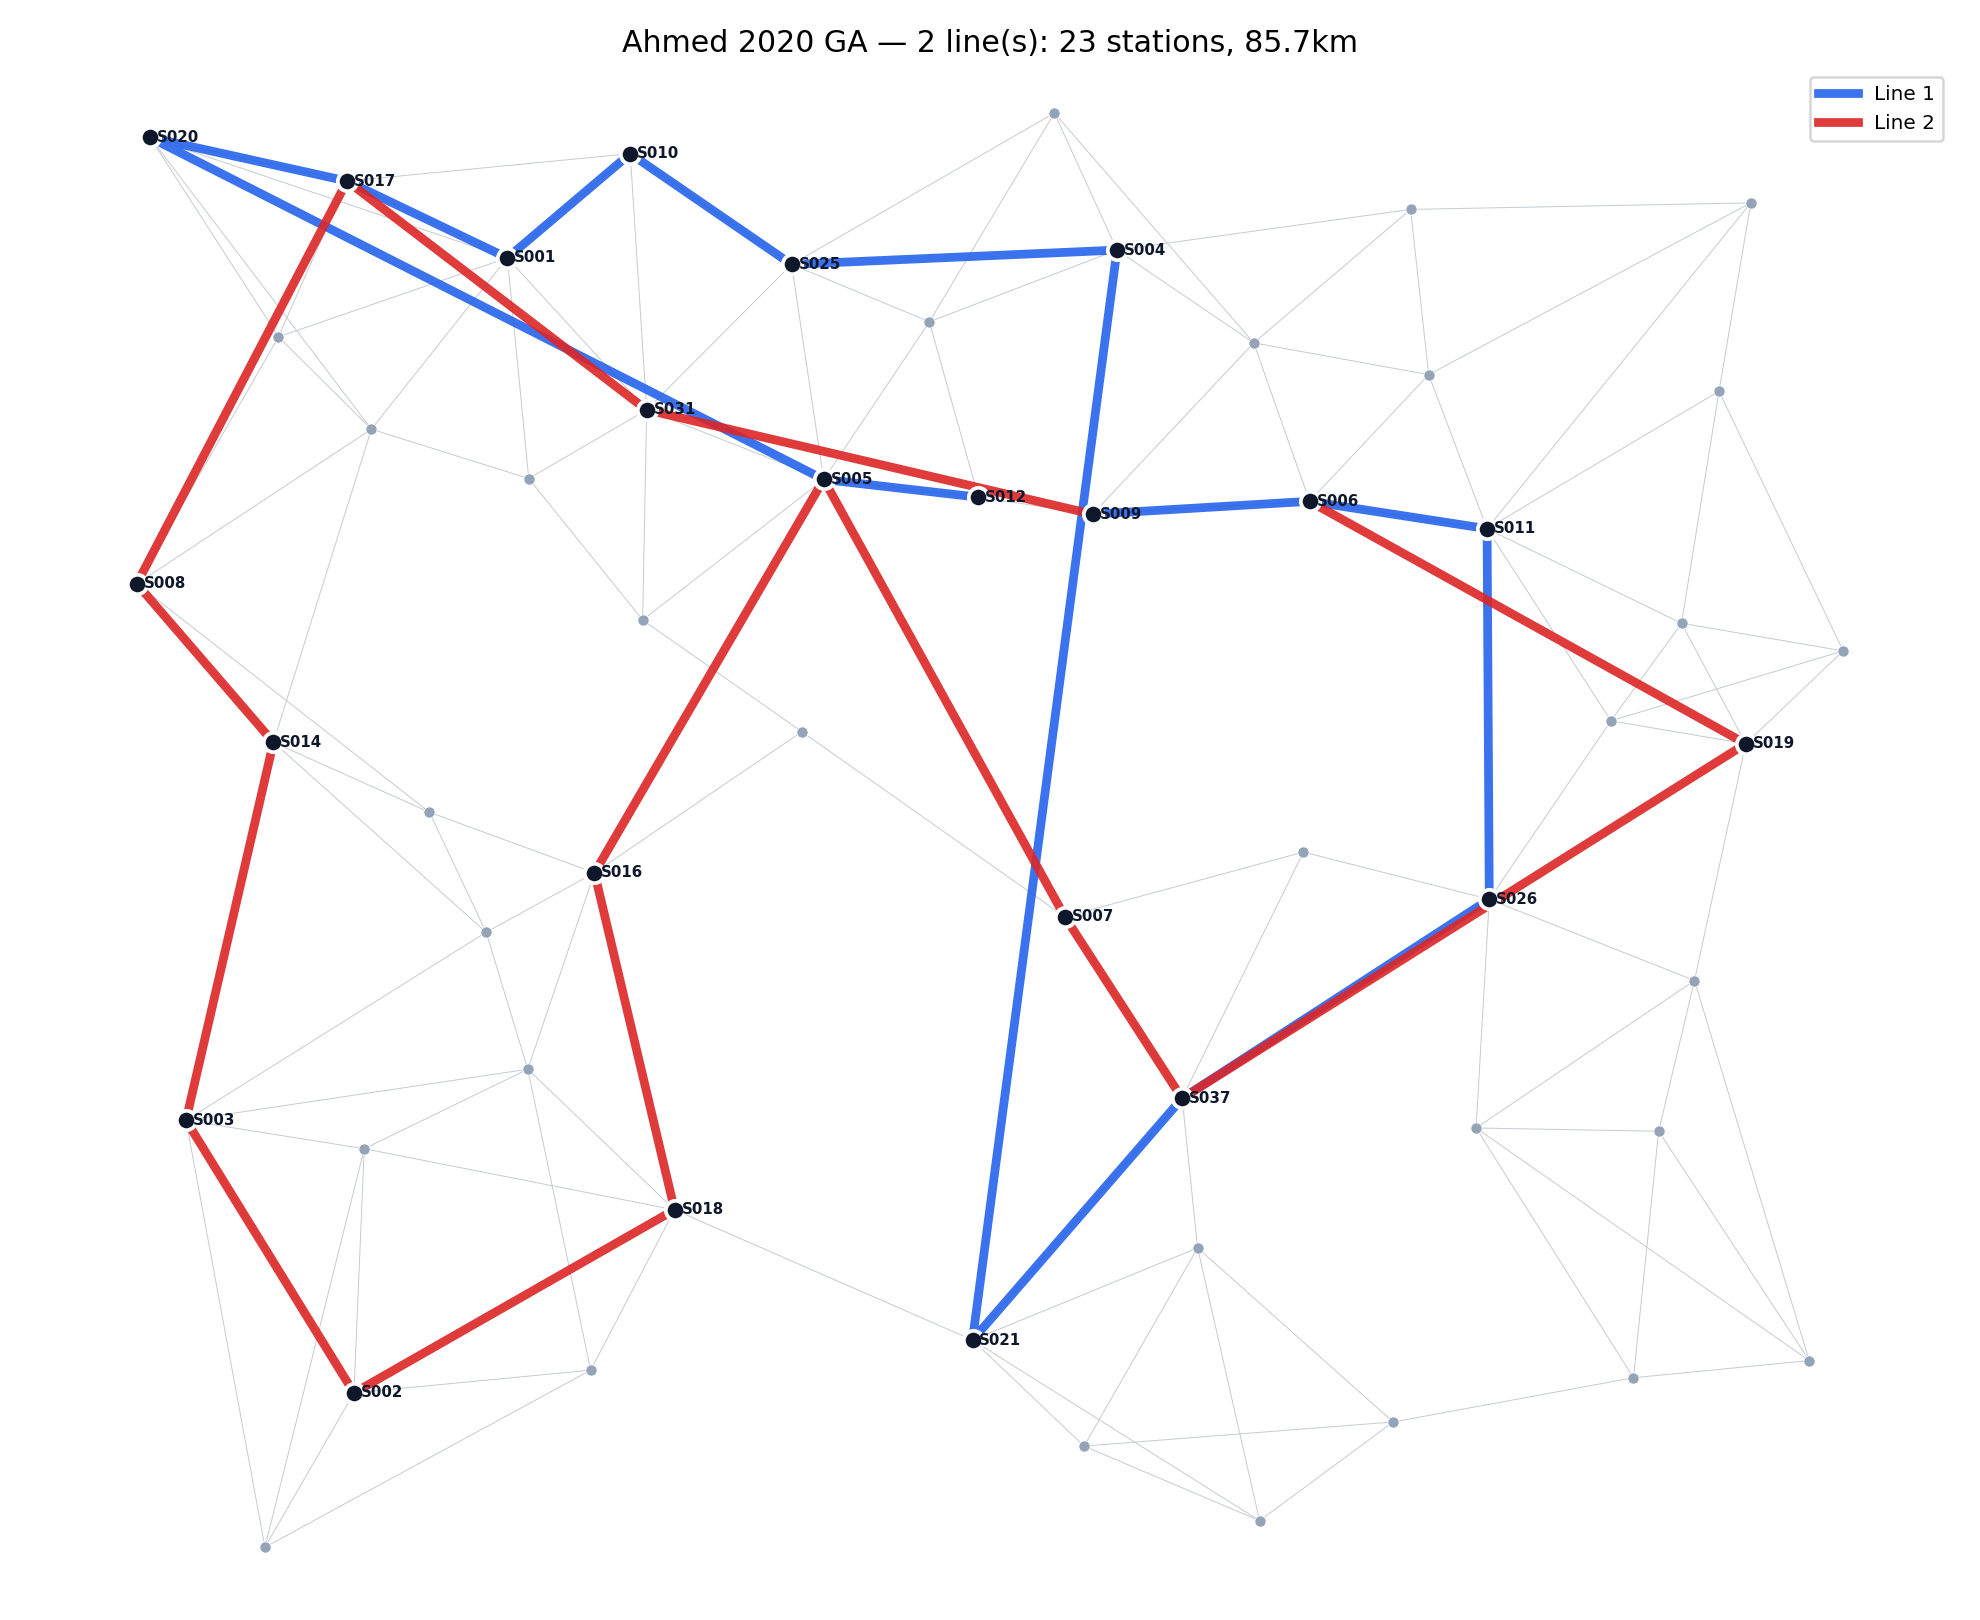
\includegraphics[width=\linewidth, height=14cm]{ahmed2020_reproduction/network_2line}
\end{minipage}\hfill
\begin{minipage}{0.31\linewidth}\centering
\Large\textbf{3-line network}\\[0.1cm]
20 stations, 130.8 km\\[0.15cm]
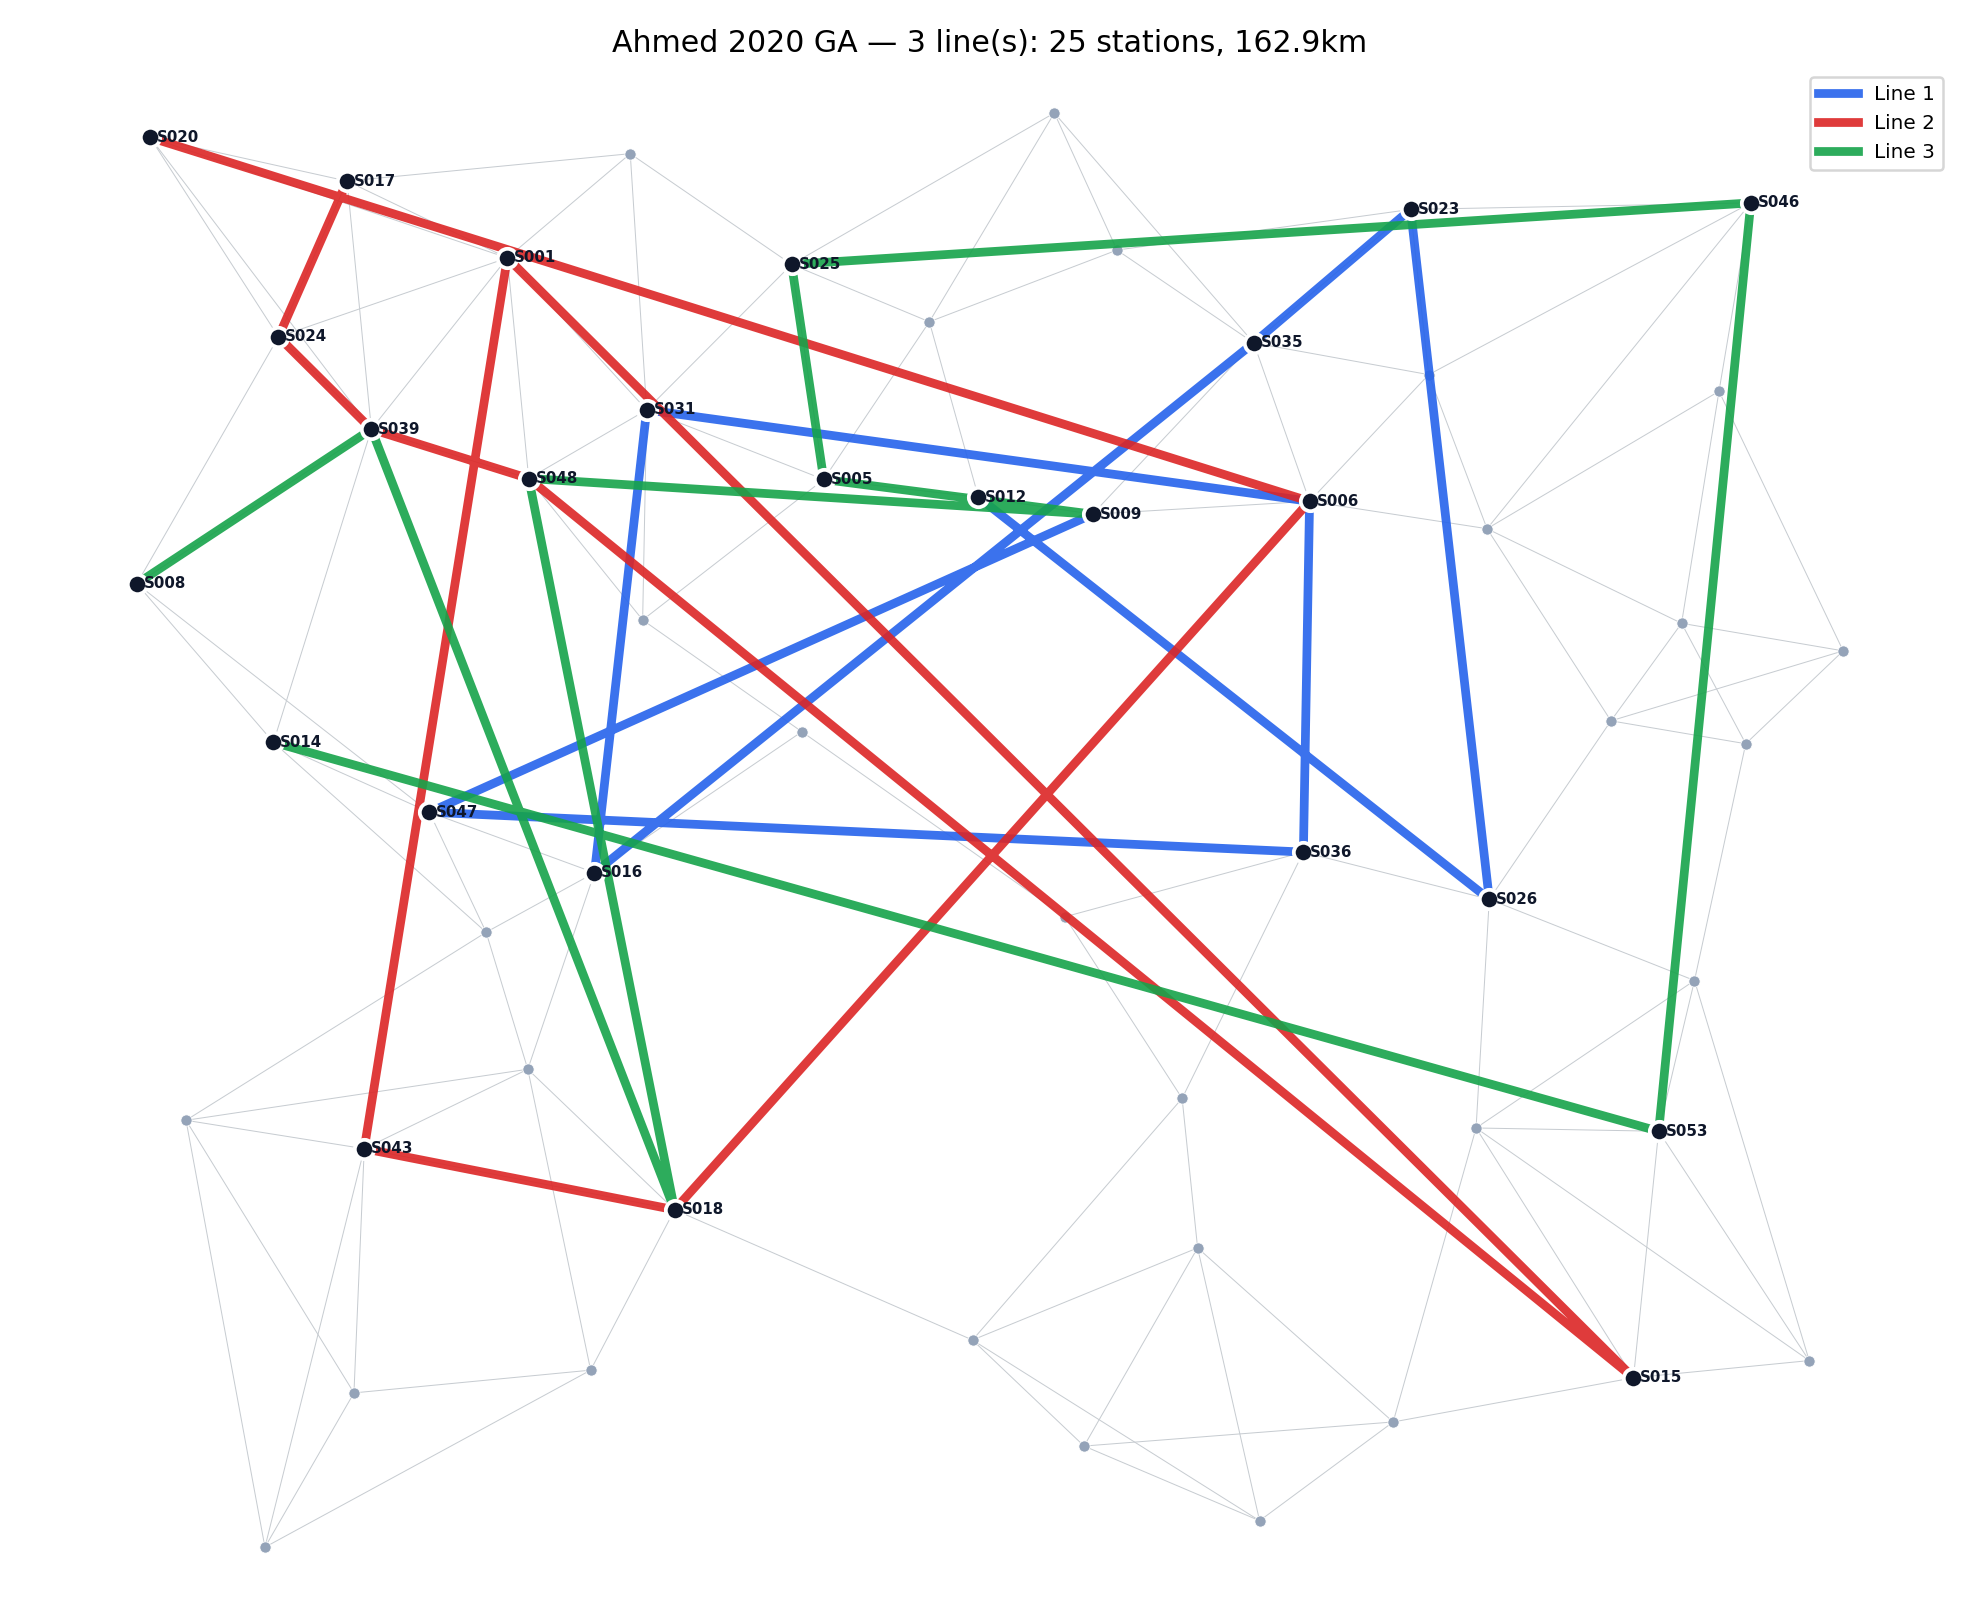
\includegraphics[width=\linewidth, height=14cm]{ahmed2020_reproduction/network_3line}
\end{minipage}
\end{center}
\vspace{0.1cm}
{\normalsize The 2-line network establishes \textbf{5 transfer stations} enabling cross-line passenger flows. The 3-line network adds southern corridor coverage but at higher construction cost with diminishing OD returns.}
\end{block}

\vspace{0.2cm}

% --- SENSITIVITY + SIMULTANEOUS ---
\begin{block}{\Large Sensitivity Analysis \& Simultaneous vs.\ Individual}
\normalsize
\begin{minipage}{0.52\linewidth}
\textbf{Spacing sensitivity:} Varying min inter-station spacing from 500m to 1500m. The original paper claims H1 dominates for $\geq$1250m; on our denser 54-station set, H2-A consistently outperforms H1 at all spacings.

\textbf{Runtime scalability:} H1 $\sim$0.8s, H2 $\sim$20s at $n{=}100$. H1 is \textbf{25$\times$ faster}, confirming $O(n^2)$ vs.\ $O(n^3)$.

\vspace{0.15cm}
\begin{center}
\begin{minipage}{0.47\linewidth}\centering
\normalsize\textbf{Spacing Sensitivity}\\[0.1cm]
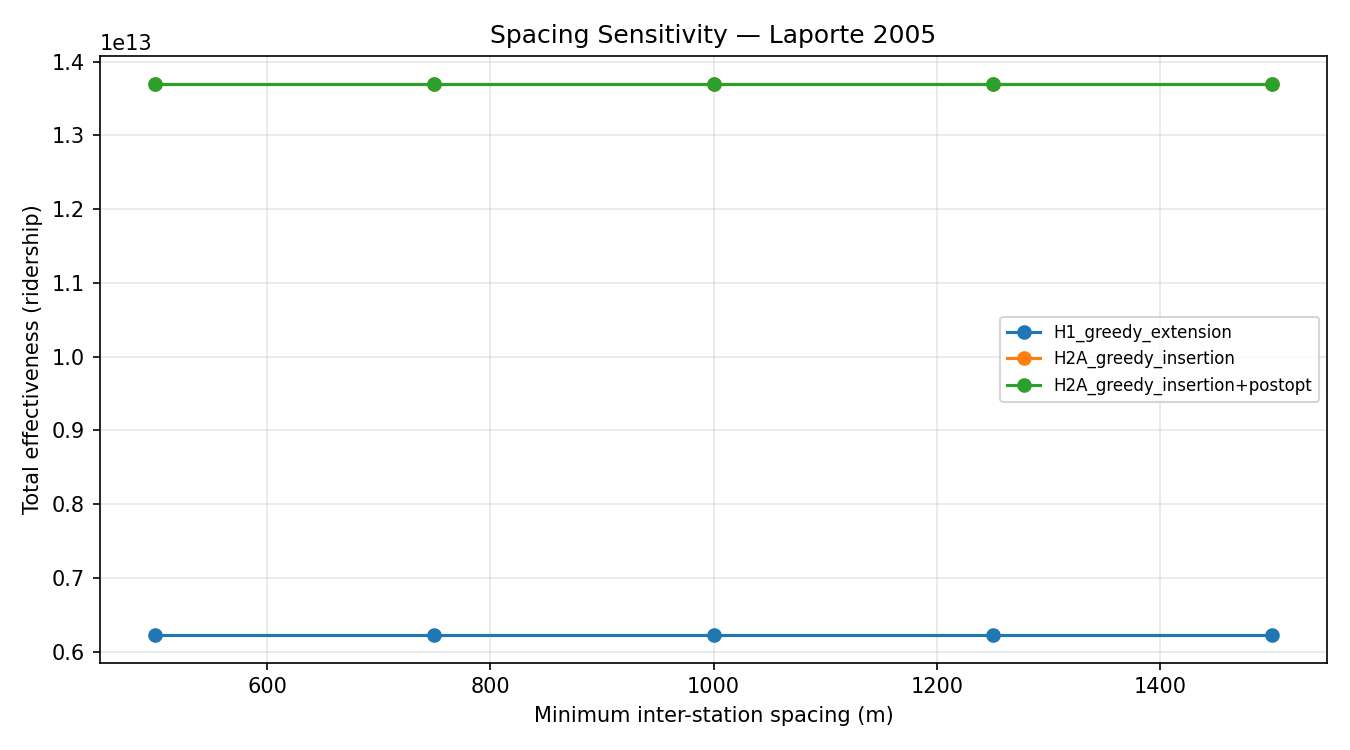
\includegraphics[height=5cm]{laporte2005_reproduction/spacing_sensitivity}
\end{minipage}\hfill
\begin{minipage}{0.47\linewidth}\centering
\normalsize\textbf{Runtime Scalability}\\[0.1cm]
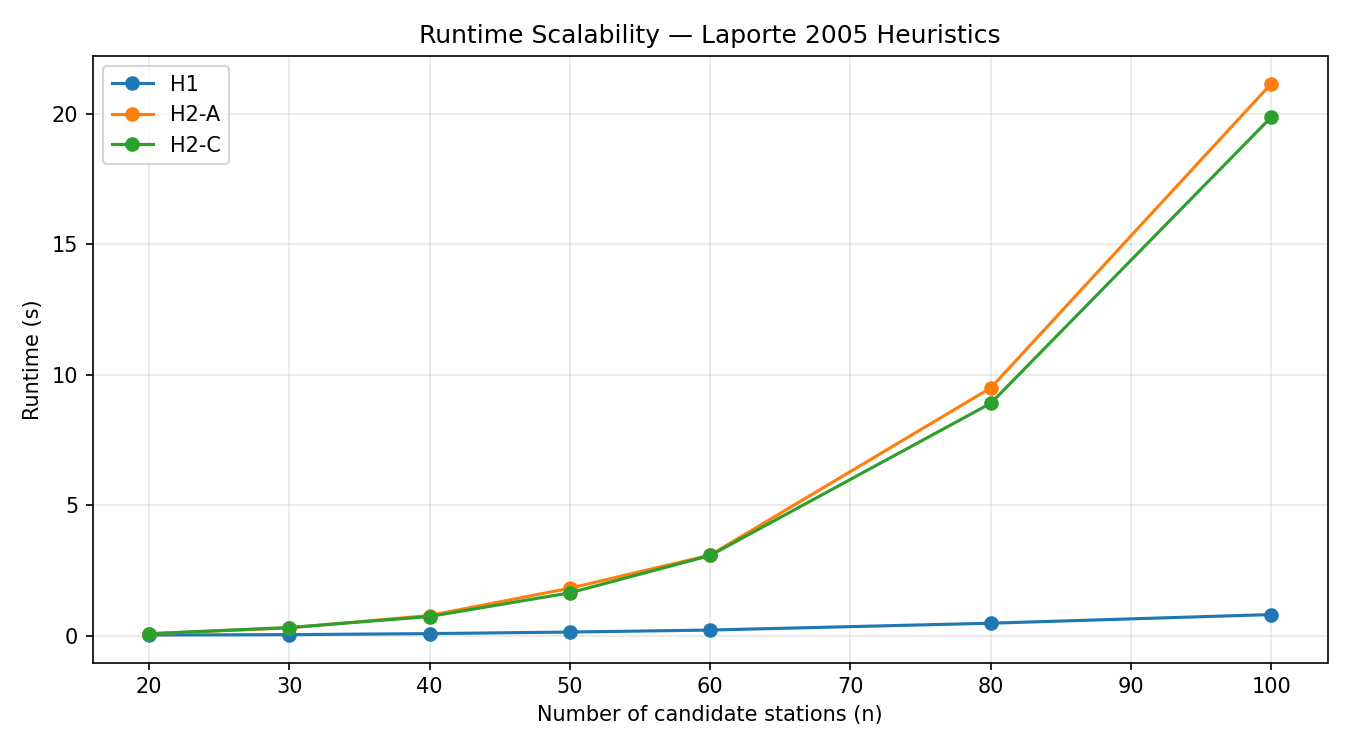
\includegraphics[height=5cm]{laporte2005_reproduction/runtime_scalability}
\end{minipage}
\end{center}
\end{minipage}\hfill
\begin{minipage}{0.45\linewidth}
\textbf{Simultaneous vs.\ Individual} (2-line scenario):

\begin{center}
\small
\begin{tabular}{@{}lcc@{}}
\toprule
& \textbf{Simult.} & \textbf{Indiv.} \\
\midrule
Total cost & $-1.33\mathrm{e}13$ & $-1.13\mathrm{e}13$ \\
Stations & 23 & 28 \\
Length (km) & 85.7 & 80.1 \\
Runtime (s) & 58.3 & 68.9 \\
\midrule
\multicolumn{3}{c}{\textbf{18\% better cost, 5 fewer stn}} \\
\bottomrule
\end{tabular}
\end{center}

\vspace{0.1cm}
Simultaneous optimization achieves \textbf{18\% lower total cost} while using 5 fewer stations, by coordinating line routing and transfer placement globally. The original paper reports 70\%; gap due to simplified cost model (54 vs.\ 4774 cells).
\end{minipage}
\end{block}

\end{minipage}

\vspace{0.15cm}

% ================================================================
%  FOOTER
% ================================================================
\begin{beamercolorbox}[wd=\paperwidth, center, sep=0.2cm]{footline}
{\fontsize{11}{14}\selectfont\color{white} Code: \texttt{Rail-Line-Planning/line\_network\_model} \quad$\vert$\quad
ShanghaiTech University, CS240 Spring 2026}
\end{beamercolorbox}

\end{frame}
\end{document}
